\documentclass[twoside]{book}

% Packages required by doxygen
\usepackage{fixltx2e}
\usepackage{calc}
\usepackage{doxygen}
\usepackage[export]{adjustbox} % also loads graphicx
\usepackage{graphicx}
\usepackage[utf8]{inputenc}
\usepackage{makeidx}
\usepackage{multicol}
\usepackage{multirow}
\PassOptionsToPackage{warn}{textcomp}
\usepackage{textcomp}
\usepackage[nointegrals]{wasysym}
\usepackage[table]{xcolor}

% Font selection
\usepackage[T1]{fontenc}
\usepackage[scaled=.90]{helvet}
\usepackage{courier}
\usepackage{amssymb}
\usepackage{sectsty}
\renewcommand{\familydefault}{\sfdefault}
\allsectionsfont{%
  \fontseries{bc}\selectfont%
  \color{darkgray}%
}
\renewcommand{\DoxyLabelFont}{%
  \fontseries{bc}\selectfont%
  \color{darkgray}%
}
\newcommand{\+}{\discretionary{\mbox{\scriptsize$\hookleftarrow$}}{}{}}

% Page & text layout
\usepackage{geometry}
\geometry{%
  a4paper,%
  top=2.5cm,%
  bottom=2.5cm,%
  left=2.5cm,%
  right=2.5cm%
}
\tolerance=750
\hfuzz=15pt
\hbadness=750
\setlength{\emergencystretch}{15pt}
\setlength{\parindent}{0cm}
\setlength{\parskip}{3ex plus 2ex minus 2ex}
\makeatletter
\renewcommand{\paragraph}{%
  \@startsection{paragraph}{4}{0ex}{-1.0ex}{1.0ex}{%
    \normalfont\normalsize\bfseries\SS@parafont%
  }%
}
\renewcommand{\subparagraph}{%
  \@startsection{subparagraph}{5}{0ex}{-1.0ex}{1.0ex}{%
    \normalfont\normalsize\bfseries\SS@subparafont%
  }%
}
\makeatother

% Headers & footers
\usepackage{fancyhdr}
\pagestyle{fancyplain}
\fancyhead[LE]{\fancyplain{}{\bfseries\thepage}}
\fancyhead[CE]{\fancyplain{}{}}
\fancyhead[RE]{\fancyplain{}{\bfseries\leftmark}}
\fancyhead[LO]{\fancyplain{}{\bfseries\rightmark}}
\fancyhead[CO]{\fancyplain{}{}}
\fancyhead[RO]{\fancyplain{}{\bfseries\thepage}}
\fancyfoot[LE]{\fancyplain{}{}}
\fancyfoot[CE]{\fancyplain{}{}}
\fancyfoot[RE]{\fancyplain{}{\bfseries\scriptsize Generated by Doxygen }}
\fancyfoot[LO]{\fancyplain{}{\bfseries\scriptsize Generated by Doxygen }}
\fancyfoot[CO]{\fancyplain{}{}}
\fancyfoot[RO]{\fancyplain{}{}}
\renewcommand{\footrulewidth}{0.4pt}
\renewcommand{\chaptermark}[1]{%
  \markboth{#1}{}%
}
\renewcommand{\sectionmark}[1]{%
  \markright{\thesection\ #1}%
}

% Indices & bibliography
\usepackage{natbib}
\usepackage[titles]{tocloft}
\setcounter{tocdepth}{3}
\setcounter{secnumdepth}{5}
\makeindex

% Hyperlinks (required, but should be loaded last)
\usepackage{ifpdf}
\ifpdf
  \usepackage[pdftex,pagebackref=true]{hyperref}
\else
  \usepackage[ps2pdf,pagebackref=true]{hyperref}
\fi
\hypersetup{%
  colorlinks=true,%
  linkcolor=blue,%
  citecolor=blue,%
  unicode%
}

% Custom commands
\newcommand{\clearemptydoublepage}{%
  \newpage{\pagestyle{empty}\cleardoublepage}%
}

\usepackage{caption}
\captionsetup{labelsep=space,justification=centering,font={bf},singlelinecheck=off,skip=4pt,position=top}

%===== C O N T E N T S =====

\begin{document}

% Titlepage & ToC
\hypersetup{pageanchor=false,
             bookmarksnumbered=true,
             pdfencoding=unicode
            }
\pagenumbering{roman}
\begin{titlepage}
\vspace*{7cm}
\begin{center}%
{\Large My Project }\\
\vspace*{1cm}
{\large Generated by Doxygen 1.8.11}\\
\end{center}
\end{titlepage}
\clearemptydoublepage
\tableofcontents
\clearemptydoublepage
\pagenumbering{arabic}
\hypersetup{pageanchor=true}

%--- Begin generated contents ---
\chapter{Hierarchical Index}
\section{Class Hierarchy}
This inheritance list is sorted roughly, but not completely, alphabetically\+:\begin{DoxyCompactList}
\item \contentsline{section}{collect}{\pageref{classcollect}}{}
\item \contentsline{section}{out\+\_\+base}{\pageref{classout__base}}{}
\begin{DoxyCompactList}
\item \contentsline{section}{log\+\_\+out}{\pageref{classlog__out}}{}
\item \contentsline{section}{write\+\_\+out}{\pageref{classwrite__out}}{}
\end{DoxyCompactList}
\item \contentsline{section}{report}{\pageref{classreport}}{}
\end{DoxyCompactList}

\chapter{Class Index}
\section{Class List}
Here are the classes, structs, unions and interfaces with brief descriptions\+:\begin{DoxyCompactList}
\item\contentsline{section}{\hyperlink{classcollect}{collect} }{\pageref{classcollect}}{}
\item\contentsline{section}{\hyperlink{classlog__out}{log\+\_\+out} }{\pageref{classlog__out}}{}
\item\contentsline{section}{\hyperlink{classout__base}{out\+\_\+base} }{\pageref{classout__base}}{}
\item\contentsline{section}{\hyperlink{classreport}{report} }{\pageref{classreport}}{}
\item\contentsline{section}{\hyperlink{classwrite__out}{write\+\_\+out} }{\pageref{classwrite__out}}{}
\end{DoxyCompactList}

\chapter{File Index}
\section{File List}
Here is a list of all files with brief descriptions\+:\begin{DoxyCompactList}
\item\contentsline{section}{\hyperlink{class__out_8h}{class\+\_\+out.\+h} }{\pageref{class__out_8h}}{}
\item\contentsline{section}{\hyperlink{collect_8cpp}{collect.\+cpp} }{\pageref{collect_8cpp}}{}
\item\contentsline{section}{\hyperlink{collect_8h}{collect.\+h} }{\pageref{collect_8h}}{}
\item\contentsline{section}{\hyperlink{main_8cpp}{main.\+cpp} }{\pageref{main_8cpp}}{}
\item\contentsline{section}{\hyperlink{user__types_8h}{user\+\_\+types.\+h} }{\pageref{user__types_8h}}{}
\end{DoxyCompactList}

\chapter{Class Documentation}
\hypertarget{classcollect}{}\section{collect Class Reference}
\label{classcollect}\index{collect@{collect}}


{\ttfamily \#include $<$collect.\+h$>$}

\subsection*{Public Member Functions}
\begin{DoxyCompactItemize}
\item 
\hyperlink{classcollect_a6b0d8b16c74fff287645a9b85dbfb68f}{collect} (unsigned int n)
\item 
\hyperlink{collect_8h_a0366ca6af63a79df33b7bb52876a5d0a}{res\+\_\+t} \hyperlink{classcollect_a08cbe31fb7b3c98d43f78ae39f1ad589}{handle} (std\+::string str)
\item 
\hyperlink{collect_8h_a0366ca6af63a79df33b7bb52876a5d0a}{res\+\_\+t} \hyperlink{classcollect_a553cfc8b8f7791a990e08747bd2052ca}{get\+\_\+now} ()
\end{DoxyCompactItemize}


\subsection{Constructor \& Destructor Documentation}
\index{collect@{collect}!collect@{collect}}
\index{collect@{collect}!collect@{collect}}
\subsubsection[{\texorpdfstring{collect(unsigned int n)}{collect(unsigned int n)}}]{\setlength{\rightskip}{0pt plus 5cm}collect\+::collect (
\begin{DoxyParamCaption}
\item[{unsigned int}]{n}
\end{DoxyParamCaption}
)}\hypertarget{classcollect_a6b0d8b16c74fff287645a9b85dbfb68f}{}\label{classcollect_a6b0d8b16c74fff287645a9b85dbfb68f}


\subsection{Member Function Documentation}
\index{collect@{collect}!get\+\_\+now@{get\+\_\+now}}
\index{get\+\_\+now@{get\+\_\+now}!collect@{collect}}
\subsubsection[{\texorpdfstring{get\+\_\+now()}{get_now()}}]{\setlength{\rightskip}{0pt plus 5cm}{\bf res\+\_\+t} collect\+::get\+\_\+now (
\begin{DoxyParamCaption}
{}
\end{DoxyParamCaption}
)}\hypertarget{classcollect_a553cfc8b8f7791a990e08747bd2052ca}{}\label{classcollect_a553cfc8b8f7791a990e08747bd2052ca}
\index{collect@{collect}!handle@{handle}}
\index{handle@{handle}!collect@{collect}}
\subsubsection[{\texorpdfstring{handle(std\+::string str)}{handle(std::string str)}}]{\setlength{\rightskip}{0pt plus 5cm}{\bf res\+\_\+t} collect\+::handle (
\begin{DoxyParamCaption}
\item[{std\+::string}]{str}
\end{DoxyParamCaption}
)}\hypertarget{classcollect_a08cbe31fb7b3c98d43f78ae39f1ad589}{}\label{classcollect_a08cbe31fb7b3c98d43f78ae39f1ad589}


The documentation for this class was generated from the following files\+:\begin{DoxyCompactItemize}
\item 
\hyperlink{collect_8h}{collect.\+h}\item 
\hyperlink{collect_8cpp}{collect.\+cpp}\end{DoxyCompactItemize}

\hypertarget{classlog__out}{}\section{log\+\_\+out Class Reference}
\label{classlog__out}\index{log\+\_\+out@{log\+\_\+out}}


{\ttfamily \#include $<$class\+\_\+out.\+h$>$}



Inheritance diagram for log\+\_\+out\+:
\nopagebreak
\begin{figure}[H]
\begin{center}
\leavevmode
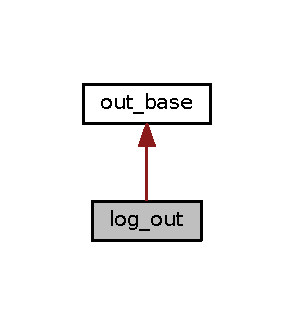
\includegraphics[width=141pt]{classlog__out__inherit__graph}
\end{center}
\end{figure}


Collaboration diagram for log\+\_\+out\+:
\nopagebreak
\begin{figure}[H]
\begin{center}
\leavevmode
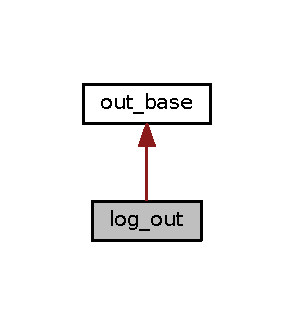
\includegraphics[width=141pt]{classlog__out__coll__graph}
\end{center}
\end{figure}
\subsection*{Public Member Functions}
\begin{DoxyCompactItemize}
\item 
\hyperlink{classlog__out_a566584f3c9ed27109893556c022bab13}{log\+\_\+out} (\hyperlink{classreport}{report} $\ast$rp)
\item 
void \hyperlink{classlog__out_a875e78afb368e28caaf4e992bfce25b6}{write} (\hyperlink{user__types_8h_ab91e48949abe3320051cfa7e864287a0}{cmd\+\_\+list\+\_\+t} val, \hyperlink{user__types_8h_a1696a9e652482a90f0c5e1c7d0eb5c61}{time\+\_\+point\+\_\+t}) override
\end{DoxyCompactItemize}


\subsection{Constructor \& Destructor Documentation}
\index{log\+\_\+out@{log\+\_\+out}!log\+\_\+out@{log\+\_\+out}}
\index{log\+\_\+out@{log\+\_\+out}!log\+\_\+out@{log\+\_\+out}}
\subsubsection[{\texorpdfstring{log\+\_\+out(report $\ast$rp)}{log_out(report *rp)}}]{\setlength{\rightskip}{0pt plus 5cm}log\+\_\+out\+::log\+\_\+out (
\begin{DoxyParamCaption}
\item[{{\bf report} $\ast$}]{rp}
\end{DoxyParamCaption}
)}\hypertarget{classlog__out_a566584f3c9ed27109893556c022bab13}{}\label{classlog__out_a566584f3c9ed27109893556c022bab13}


\subsection{Member Function Documentation}
\index{log\+\_\+out@{log\+\_\+out}!write@{write}}
\index{write@{write}!log\+\_\+out@{log\+\_\+out}}
\subsubsection[{\texorpdfstring{write(cmd\+\_\+list\+\_\+t val, time\+\_\+point\+\_\+t) override}{write(cmd_list_t val, time_point_t) override}}]{\setlength{\rightskip}{0pt plus 5cm}void log\+\_\+out\+::write (
\begin{DoxyParamCaption}
\item[{{\bf cmd\+\_\+list\+\_\+t}}]{val, }
\item[{{\bf time\+\_\+point\+\_\+t}}]{}
\end{DoxyParamCaption}
)\hspace{0.3cm}{\ttfamily [inline]}, {\ttfamily [override]}, {\ttfamily [virtual]}}\hypertarget{classlog__out_a875e78afb368e28caaf4e992bfce25b6}{}\label{classlog__out_a875e78afb368e28caaf4e992bfce25b6}


Implements \hyperlink{classout__base_a3ee9ed833bd3e2620cea18e1bc90b352}{out\+\_\+base}.



The documentation for this class was generated from the following file\+:\begin{DoxyCompactItemize}
\item 
\hyperlink{class__out_8h}{class\+\_\+out.\+h}\end{DoxyCompactItemize}

\hypertarget{classout__base}{}\section{out\+\_\+base Class Reference}
\label{classout__base}\index{out\+\_\+base@{out\+\_\+base}}


{\ttfamily \#include $<$class\+\_\+out.\+h$>$}



Inheritance diagram for out\+\_\+base\+:
% FIG 0
\subsection*{Public Member Functions}
\begin{DoxyCompactItemize}
\item 
virtual \hyperlink{classout__base_af3709ed0192c02cbdfb4373c19f79178}{$\sim$out\+\_\+base} ()=default
\item 
virtual void \hyperlink{classout__base_a3ee9ed833bd3e2620cea18e1bc90b352}{write} (\hyperlink{user__types_8h_ab91e48949abe3320051cfa7e864287a0}{cmd\+\_\+list\+\_\+t} str, \hyperlink{user__types_8h_a1696a9e652482a90f0c5e1c7d0eb5c61}{time\+\_\+point\+\_\+t} tp)=0
\end{DoxyCompactItemize}


\subsection{Constructor \& Destructor Documentation}
\index{out\+\_\+base@{out\+\_\+base}!````~out\+\_\+base@{$\sim$out\+\_\+base}}
\index{````~out\+\_\+base@{$\sim$out\+\_\+base}!out\+\_\+base@{out\+\_\+base}}
\subsubsection[{\texorpdfstring{$\sim$out\+\_\+base()=default}{~out_base()=default}}]{\setlength{\rightskip}{0pt plus 5cm}virtual out\+\_\+base\+::$\sim$out\+\_\+base (
\begin{DoxyParamCaption}
{}
\end{DoxyParamCaption}
)\hspace{0.3cm}{\ttfamily [virtual]}, {\ttfamily [default]}}\hypertarget{classout__base_af3709ed0192c02cbdfb4373c19f79178}{}\label{classout__base_af3709ed0192c02cbdfb4373c19f79178}


\subsection{Member Function Documentation}
\index{out\+\_\+base@{out\+\_\+base}!write@{write}}
\index{write@{write}!out\+\_\+base@{out\+\_\+base}}
\subsubsection[{\texorpdfstring{write(cmd\+\_\+list\+\_\+t str, time\+\_\+point\+\_\+t tp)=0}{write(cmd_list_t str, time_point_t tp)=0}}]{\setlength{\rightskip}{0pt plus 5cm}virtual void out\+\_\+base\+::write (
\begin{DoxyParamCaption}
\item[{{\bf cmd\+\_\+list\+\_\+t}}]{str, }
\item[{{\bf time\+\_\+point\+\_\+t}}]{tp}
\end{DoxyParamCaption}
)\hspace{0.3cm}{\ttfamily [pure virtual]}}\hypertarget{classout__base_a3ee9ed833bd3e2620cea18e1bc90b352}{}\label{classout__base_a3ee9ed833bd3e2620cea18e1bc90b352}


Implemented in \hyperlink{classwrite__out_a4a3831720d119fbda93b690979ea3538}{write\+\_\+out}, and \hyperlink{classlog__out_a875e78afb368e28caaf4e992bfce25b6}{log\+\_\+out}.



The documentation for this class was generated from the following file\+:\begin{DoxyCompactItemize}
\item 
\hyperlink{class__out_8h}{class\+\_\+out.\+h}\end{DoxyCompactItemize}

\hypertarget{classreport}{}\section{report Class Reference}
\label{classreport}\index{report@{report}}


{\ttfamily \#include $<$class\+\_\+out.\+h$>$}

\subsection*{Public Member Functions}
\begin{DoxyCompactItemize}
\item 
void \hyperlink{classreport_a18f9439720a91f3d7fce9ac32947a538}{subscribe} (\hyperlink{classout__base}{out\+\_\+base} $\ast$ptr)
\item 
void \hyperlink{classreport_aefe211b52c3ad1f245388b40cc799514}{notify\+\_\+all} (\hyperlink{user__types_8h_ab91e48949abe3320051cfa7e864287a0}{cmd\+\_\+list\+\_\+t} val, \hyperlink{user__types_8h_a1696a9e652482a90f0c5e1c7d0eb5c61}{time\+\_\+point\+\_\+t} time)
\end{DoxyCompactItemize}


\subsection{Member Function Documentation}
\index{report@{report}!notify\+\_\+all@{notify\+\_\+all}}
\index{notify\+\_\+all@{notify\+\_\+all}!report@{report}}
\subsubsection[{\texorpdfstring{notify\+\_\+all(cmd\+\_\+list\+\_\+t val, time\+\_\+point\+\_\+t time)}{notify_all(cmd_list_t val, time_point_t time)}}]{\setlength{\rightskip}{0pt plus 5cm}void report\+::notify\+\_\+all (
\begin{DoxyParamCaption}
\item[{{\bf cmd\+\_\+list\+\_\+t}}]{val, }
\item[{{\bf time\+\_\+point\+\_\+t}}]{time}
\end{DoxyParamCaption}
)\hspace{0.3cm}{\ttfamily [inline]}}\hypertarget{classreport_aefe211b52c3ad1f245388b40cc799514}{}\label{classreport_aefe211b52c3ad1f245388b40cc799514}
\index{report@{report}!subscribe@{subscribe}}
\index{subscribe@{subscribe}!report@{report}}
\subsubsection[{\texorpdfstring{subscribe(out\+\_\+base $\ast$ptr)}{subscribe(out_base *ptr)}}]{\setlength{\rightskip}{0pt plus 5cm}void report\+::subscribe (
\begin{DoxyParamCaption}
\item[{{\bf out\+\_\+base} $\ast$}]{ptr}
\end{DoxyParamCaption}
)\hspace{0.3cm}{\ttfamily [inline]}}\hypertarget{classreport_a18f9439720a91f3d7fce9ac32947a538}{}\label{classreport_a18f9439720a91f3d7fce9ac32947a538}


The documentation for this class was generated from the following file\+:\begin{DoxyCompactItemize}
\item 
\hyperlink{class__out_8h}{class\+\_\+out.\+h}\end{DoxyCompactItemize}

\hypertarget{classwrite__out}{}\section{write\+\_\+out Class Reference}
\label{classwrite__out}\index{write\+\_\+out@{write\+\_\+out}}


{\ttfamily \#include $<$class\+\_\+out.\+h$>$}



Inheritance diagram for write\+\_\+out\+:
\nopagebreak
\begin{figure}[H]
\begin{center}
\leavevmode
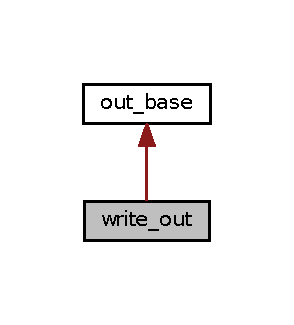
\includegraphics[width=141pt]{classwrite__out__inherit__graph}
\end{center}
\end{figure}


Collaboration diagram for write\+\_\+out\+:
\nopagebreak
\begin{figure}[H]
\begin{center}
\leavevmode
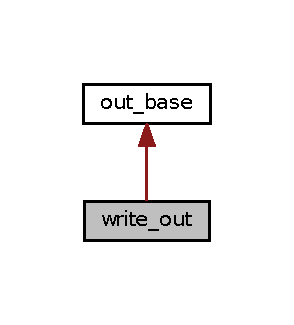
\includegraphics[width=141pt]{classwrite__out__coll__graph}
\end{center}
\end{figure}
\subsection*{Public Member Functions}
\begin{DoxyCompactItemize}
\item 
\hyperlink{classwrite__out_a5516dbcc50bdf9cdfc70824a7aab75dd}{write\+\_\+out} (\hyperlink{classreport}{report} $\ast$rp)
\item 
void \hyperlink{classwrite__out_a4a3831720d119fbda93b690979ea3538}{write} (\hyperlink{user__types_8h_ab91e48949abe3320051cfa7e864287a0}{cmd\+\_\+list\+\_\+t} val, \hyperlink{user__types_8h_a1696a9e652482a90f0c5e1c7d0eb5c61}{time\+\_\+point\+\_\+t} tp) override
\end{DoxyCompactItemize}


\subsection{Constructor \& Destructor Documentation}
\index{write\+\_\+out@{write\+\_\+out}!write\+\_\+out@{write\+\_\+out}}
\index{write\+\_\+out@{write\+\_\+out}!write\+\_\+out@{write\+\_\+out}}
\subsubsection[{\texorpdfstring{write\+\_\+out(report $\ast$rp)}{write_out(report *rp)}}]{\setlength{\rightskip}{0pt plus 5cm}write\+\_\+out\+::write\+\_\+out (
\begin{DoxyParamCaption}
\item[{{\bf report} $\ast$}]{rp}
\end{DoxyParamCaption}
)}\hypertarget{classwrite__out_a5516dbcc50bdf9cdfc70824a7aab75dd}{}\label{classwrite__out_a5516dbcc50bdf9cdfc70824a7aab75dd}


\subsection{Member Function Documentation}
\index{write\+\_\+out@{write\+\_\+out}!write@{write}}
\index{write@{write}!write\+\_\+out@{write\+\_\+out}}
\subsubsection[{\texorpdfstring{write(cmd\+\_\+list\+\_\+t val, time\+\_\+point\+\_\+t tp) override}{write(cmd_list_t val, time_point_t tp) override}}]{\setlength{\rightskip}{0pt plus 5cm}void write\+\_\+out\+::write (
\begin{DoxyParamCaption}
\item[{{\bf cmd\+\_\+list\+\_\+t}}]{val, }
\item[{{\bf time\+\_\+point\+\_\+t}}]{tp}
\end{DoxyParamCaption}
)\hspace{0.3cm}{\ttfamily [inline]}, {\ttfamily [override]}, {\ttfamily [virtual]}}\hypertarget{classwrite__out_a4a3831720d119fbda93b690979ea3538}{}\label{classwrite__out_a4a3831720d119fbda93b690979ea3538}


Implements \hyperlink{classout__base_a3ee9ed833bd3e2620cea18e1bc90b352}{out\+\_\+base}.



The documentation for this class was generated from the following file\+:\begin{DoxyCompactItemize}
\item 
\hyperlink{class__out_8h}{class\+\_\+out.\+h}\end{DoxyCompactItemize}

\chapter{File Documentation}
\hypertarget{class__out_8h}{}\section{class\+\_\+out.\+h File Reference}
\label{class__out_8h}\index{class\+\_\+out.\+h@{class\+\_\+out.\+h}}
{\ttfamily \#include $<$iostream$>$}\\*
{\ttfamily \#include $<$fstream$>$}\\*
{\ttfamily \#include \char`\"{}user\+\_\+types.\+h\char`\"{}}\\*
Include dependency graph for class\+\_\+out.\+h\+:

\hypertarget{collect_8cpp}{}\section{collect.\+cpp File Reference}
\label{collect_8cpp}\index{collect.\+cpp@{collect.\+cpp}}
{\ttfamily \#include \char`\"{}collect.\+h\char`\"{}}\\*
Include dependency graph for collect.\+cpp\+:
% FIG 0

\hypertarget{collect_8h}{}\section{collect.\+h File Reference}
\label{collect_8h}\index{collect.\+h@{collect.\+h}}
{\ttfamily \#include $<$optional$>$}\\*
{\ttfamily \#include \char`\"{}user\+\_\+types.\+h\char`\"{}}\\*
Include dependency graph for collect.\+h\+:
% FIG 0
This graph shows which files directly or indirectly include this file\+:
% FIG 1
\subsection*{Classes}
\begin{DoxyCompactItemize}
\item 
class \hyperlink{classcollect}{collect}
\end{DoxyCompactItemize}
\subsection*{Typedefs}
\begin{DoxyCompactItemize}
\item 
using \hyperlink{collect_8h_a0366ca6af63a79df33b7bb52876a5d0a}{res\+\_\+t} = std\+::optional$<$ std\+::pair$<$ \hyperlink{user__types_8h_ab91e48949abe3320051cfa7e864287a0}{cmd\+\_\+list\+\_\+t}, \hyperlink{user__types_8h_a1696a9e652482a90f0c5e1c7d0eb5c61}{time\+\_\+point\+\_\+t} $>$$>$
\end{DoxyCompactItemize}


\subsection{Typedef Documentation}
\index{collect.\+h@{collect.\+h}!res\+\_\+t@{res\+\_\+t}}
\index{res\+\_\+t@{res\+\_\+t}!collect.\+h@{collect.\+h}}
\subsubsection[{\texorpdfstring{res\+\_\+t}{res_t}}]{\setlength{\rightskip}{0pt plus 5cm}using {\bf res\+\_\+t} =  std\+::optional$<$std\+::pair$<${\bf cmd\+\_\+list\+\_\+t}, {\bf time\+\_\+point\+\_\+t}$>$$>$}\hypertarget{collect_8h_a0366ca6af63a79df33b7bb52876a5d0a}{}\label{collect_8h_a0366ca6af63a79df33b7bb52876a5d0a}

\hypertarget{main_8cpp}{}\section{main.\+cpp File Reference}
\label{main_8cpp}\index{main.\+cpp@{main.\+cpp}}
{\ttfamily \#include $<$optional$>$}\\*
{\ttfamily \#include \char`\"{}collect.\+h\char`\"{}}\\*
{\ttfamily \#include \char`\"{}class\+\_\+out.\+h\char`\"{}}\\*
Include dependency graph for main.\+cpp\+:
% FIG 0
\subsection*{Functions}
\begin{DoxyCompactItemize}
\item 
int \hyperlink{main_8cpp_a0ddf1224851353fc92bfbff6f499fa97}{main} (int argc, char $\ast$argv\mbox{[}$\,$\mbox{]})
\end{DoxyCompactItemize}


\subsection{Function Documentation}
\index{main.\+cpp@{main.\+cpp}!main@{main}}
\index{main@{main}!main.\+cpp@{main.\+cpp}}
\subsubsection[{\texorpdfstring{main(int argc, char $\ast$argv[])}{main(int argc, char *argv[])}}]{\setlength{\rightskip}{0pt plus 5cm}int main (
\begin{DoxyParamCaption}
\item[{int}]{argc, }
\item[{char $\ast$}]{argv\mbox{[}$\,$\mbox{]}}
\end{DoxyParamCaption}
)}\hypertarget{main_8cpp_a0ddf1224851353fc92bfbff6f499fa97}{}\label{main_8cpp_a0ddf1224851353fc92bfbff6f499fa97}

\hypertarget{user__types_8h}{}\section{user\+\_\+types.\+h File Reference}
\label{user__types_8h}\index{user\+\_\+types.\+h@{user\+\_\+types.\+h}}
{\ttfamily \#include $<$list$>$}\\*
{\ttfamily \#include $<$chrono$>$}\\*
{\ttfamily \#include $<$string$>$}\\*
Include dependency graph for user\+\_\+types.\+h\+:
\nopagebreak
\begin{figure}[H]
\begin{center}
\leavevmode
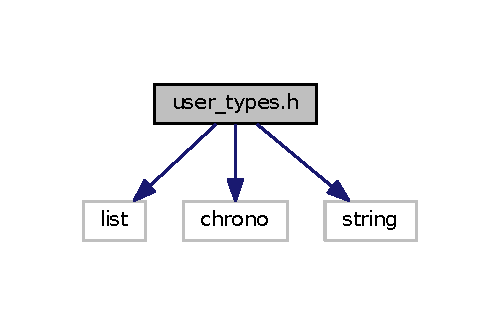
\includegraphics[width=240pt]{user__types_8h__incl}
\end{center}
\end{figure}
This graph shows which files directly or indirectly include this file\+:
\nopagebreak
\begin{figure}[H]
\begin{center}
\leavevmode
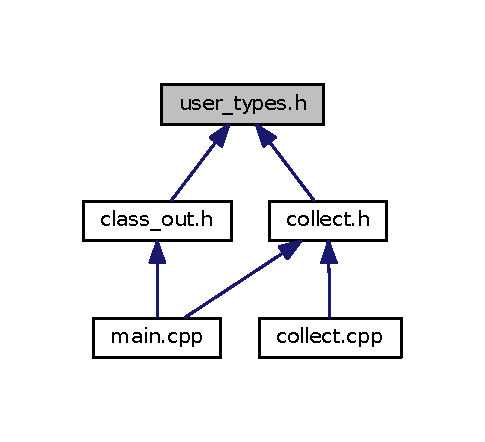
\includegraphics[width=233pt]{user__types_8h__dep__incl}
\end{center}
\end{figure}
\subsection*{Typedefs}
\begin{DoxyCompactItemize}
\item 
using \hyperlink{user__types_8h_ab91e48949abe3320051cfa7e864287a0}{cmd\+\_\+list\+\_\+t} = std\+::list$<$ std\+::string $>$
\item 
using \hyperlink{user__types_8h_a1696a9e652482a90f0c5e1c7d0eb5c61}{time\+\_\+point\+\_\+t} = std\+::chrono\+::system\+\_\+clock\+::time\+\_\+point
\end{DoxyCompactItemize}


\subsection{Typedef Documentation}
\index{user\+\_\+types.\+h@{user\+\_\+types.\+h}!cmd\+\_\+list\+\_\+t@{cmd\+\_\+list\+\_\+t}}
\index{cmd\+\_\+list\+\_\+t@{cmd\+\_\+list\+\_\+t}!user\+\_\+types.\+h@{user\+\_\+types.\+h}}
\subsubsection[{\texorpdfstring{cmd\+\_\+list\+\_\+t}{cmd_list_t}}]{\setlength{\rightskip}{0pt plus 5cm}using {\bf cmd\+\_\+list\+\_\+t} =  std\+::list$<$std\+::string$>$}\hypertarget{user__types_8h_ab91e48949abe3320051cfa7e864287a0}{}\label{user__types_8h_ab91e48949abe3320051cfa7e864287a0}
\index{user\+\_\+types.\+h@{user\+\_\+types.\+h}!time\+\_\+point\+\_\+t@{time\+\_\+point\+\_\+t}}
\index{time\+\_\+point\+\_\+t@{time\+\_\+point\+\_\+t}!user\+\_\+types.\+h@{user\+\_\+types.\+h}}
\subsubsection[{\texorpdfstring{time\+\_\+point\+\_\+t}{time_point_t}}]{\setlength{\rightskip}{0pt plus 5cm}using {\bf time\+\_\+point\+\_\+t} =  std\+::chrono\+::system\+\_\+clock\+::time\+\_\+point}\hypertarget{user__types_8h_a1696a9e652482a90f0c5e1c7d0eb5c61}{}\label{user__types_8h_a1696a9e652482a90f0c5e1c7d0eb5c61}

%--- End generated contents ---

% Index
\backmatter
\newpage
\phantomsection
\clearemptydoublepage
\addcontentsline{toc}{chapter}{Index}
\printindex

\end{document}
